\begin{figure}[t!]
    \centering
        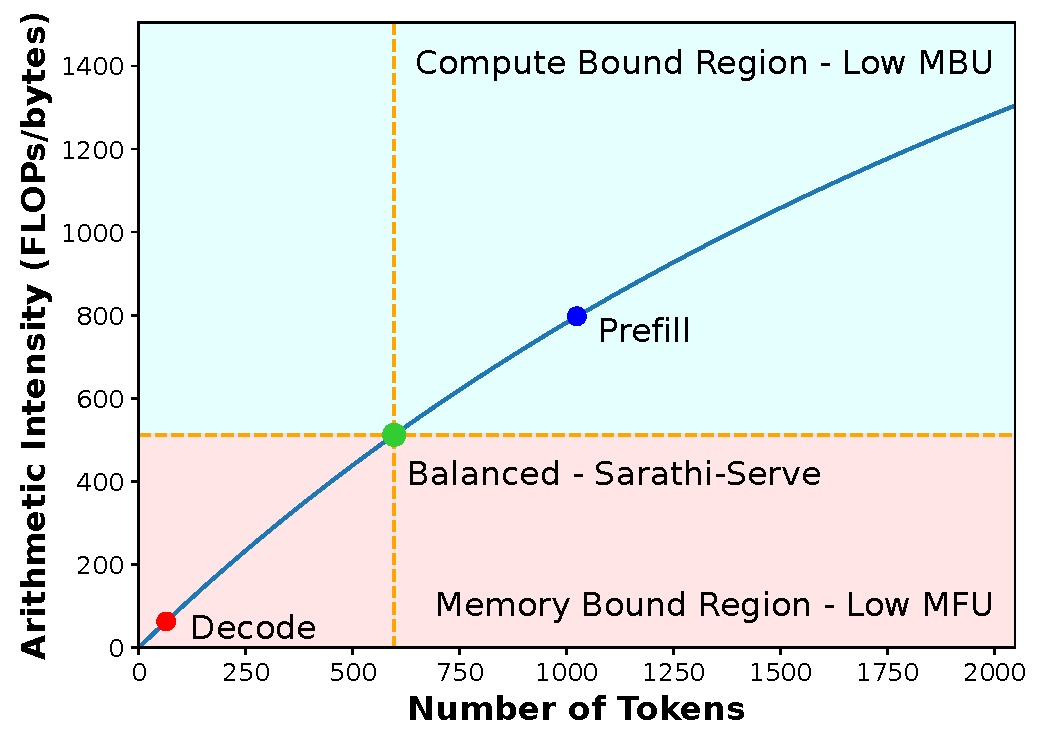
\includegraphics[width=0.45\textwidth]{figures/arithmetic_intensity.pdf}
        
    \caption{Arithmetic intensity trend for \llamaL linear operations with different number of token running on four A100s. Decode batches have low arithmetic intensity \ie they are bottlenecked by memory fetch time, leading to low compute utilization. Prefill batches are compute bound with sub-optimal bandwidth utilization. \sysname forms balanced batches by combining decodes and prefill chunks to maximize both compute and bandwidth utilization.}
       \label{fig:motivation:arithmatic-intensity}
\end{figure}
